\documentclass[14pt]{beamer}
\usepackage{./Estilos/BeamerUVM}
\usepackage{./Estilos/ColoresLatex}
\usetheme{Madrid}
\usecolortheme{default}
%\useoutertheme{default}
\setbeamercovered{invisible}
% or whatever (possibly just delete it)
\setbeamertemplate{section in toc}[sections numbered]
\setbeamertemplate{subsection in toc}[subsections numbered]
\setbeamertemplate{subsection in toc}{\leavevmode\leftskip=3.2em\rlap{\hskip-2em\inserttocsectionnumber.\inserttocsubsectionnumber}\inserttocsubsection\par}
% \setbeamercolor{section in toc}{fg=blue}
% \setbeamercolor{subsection in toc}{fg=blue}
% \setbeamercolor{frametitle}{fg=blue}
\setbeamertemplate{caption}[numbered]

\setbeamertemplate{footline}
\beamertemplatenavigationsymbolsempty
\setbeamertemplate{headline}{}


\makeatletter
% \setbeamercolor{section in foot}{bg=gray!30, fg=black!90!orange}
% \setbeamercolor{subsection in foot}{bg=blue!30}
% \setbeamercolor{date in foot}{bg=black}
\setbeamertemplate{footline}
{
  \leavevmode%
  \hbox{%
  \begin{beamercolorbox}[wd=.333333\paperwidth,ht=2.25ex,dp=1ex,center]{section in foot}%
    \usebeamerfont{section in foot} {\insertsection}
  \end{beamercolorbox}%
  \begin{beamercolorbox}[wd=.333333\paperwidth,ht=2.25ex,dp=1ex,center]{subsection in foot}%
    \usebeamerfont{subsection in foot}  \insertsubsection
  \end{beamercolorbox}%
  \begin{beamercolorbox}[wd=.333333\paperwidth,ht=2.25ex,dp=1ex,right]{date in head/foot}%
    \usebeamerfont{date in head/foot} \insertshortdate{} \hspace*{2em}
    \insertframenumber{} / \inserttotalframenumber \hspace*{2ex} 
  \end{beamercolorbox}}%
  \vskip0pt%
}
\makeatother

\makeatletter
\patchcmd{\beamer@sectionintoc}{\vskip1.5em}{\vskip0.8em}{}{}
\makeatother

% \usefonttheme{serif}
\usepackage[clock]{ifsym}
\usetikzlibrary{plotmarks}

\sisetup{per-mode=symbol}
\resetcounteronoverlays{saveenumi}

% \newcommand{\nsum}[1][1.4]{% only for \displaystyle
%     \mathop{%
%         \raisebox
%             {-#1\depthofsumsign+1\depthofsumsign}
%             {\scalebox
%                 {#1}
%                 {$\displaystyle\sum$}%
%             }
%     }
% }

\title{\Large{Leyes de movimiento} \\ \normalsize{Física 1}}
\date{24 de julio de 2023}

\begin{document}
\maketitle

\section*{Contenido}
\frame{\frametitle{Contenido} \tableofcontents[currentsection, hideallsubsections]}

% Concepto de Fuerza.
%  Tipos de fuerza
%  Vector resultante
%  Cálculo del vector resultante, magnitud y dirección.

\section{Fuerza}
\frame{\tableofcontents[currentsection, hideothersubsections]}
\subsection{Definición}

\begin{frame}
\frametitle{Experiencia diaria}
En el lenguaje cotidiano, fuerza es un empujón o un tirón.
\end{frame}
\begin{frame}
\frametitle{Definición}
Una \textocolor{byzantine}{fuerza} es una interacción entre dos cuerpos o entre un cuerpo y su ambiente.
\end{frame}
\begin{frame}
\frametitle{Fuerza como vector}
La fuerza es una cantidad vectorial, por lo que tiene una magnitud, dirección y sentido.
\begin{figure}
    \centering
    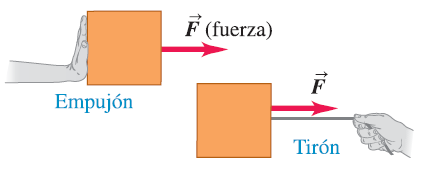
\includegraphics[scale=0.8]{Imagenes/Fuerza_01.png}
\end{figure}
\end{frame}

\subsection{Tipos de fuerza}

\begin{frame}
\frametitle{Fuerza de contacto}
Una \textocolor{cobalt}{fuerza de contacto}, es aquella fuerza que implica un contacto directo entre dos cuerpos, como un empujón o un tirón.
\end{frame}
\begin{frame}
\frametitle{Tipos de fuerza de contacto}
\setbeamercolor{item projected}{bg=bananayellow,fg=ao}
\setbeamertemplate{enumerate items}{%
\usebeamercolor[bg]{item projected}%
\raisebox{1.5pt}{\colorbox{bg}{\color{fg}\footnotesize\insertenumlabel}}%
}
\begin{enumerate}[<+->]
\item Normal.
\item Fricción.
\item Tensión.
\end{enumerate}
\end{frame}
\begin{frame}
\frametitle{Fuerza normal}
Cuando un objeto descansa o se empuja sobre una superficie, ésta ejerce un empujón sobre el objeto que \textocolor{red}{es perpendicular} a la superficie.
\pause
\begin{figure}
    \centering
    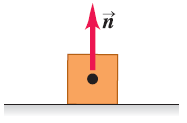
\includegraphics[scale=0.6]{Imagenes/Fuerza_02.png}
    \hspace*{1.5cm}
    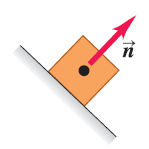
\includegraphics[scale=0.6]{Imagenes/Fuerza_03.png}
\end{figure}
\end{frame}
\begin{frame}
\frametitle{Fuerza de Fricción}
Se presenta cuando una superficie ejerce una fuerza que \textocolor{cerise}{es paralela} al objeto.
\begin{figure}
    \centering
    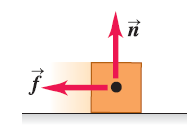
\includegraphics[scale=0.7]{Imagenes/Fuerza_04.png}
\end{figure}
\end{frame}
\begin{frame}
\frametitle{Fuerza de Tensión}
Es aquella fuerza \textocolor{cadmiumgreen}{de tirón} ejercida sobre un objeto por una cuerda, un cordón, etc.
\begin{figure}
    \centering
    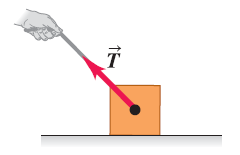
\includegraphics[scale=0.7]{Imagenes/Fuerza_05.png}
\end{figure}
\end{frame}
\begin{frame}
\frametitle{Fuerzas de largo alcance}
Son aquellas fuerzas que actúan aunque los cuerpos estén separados.
\pause
\begin{figure}
    \centering
    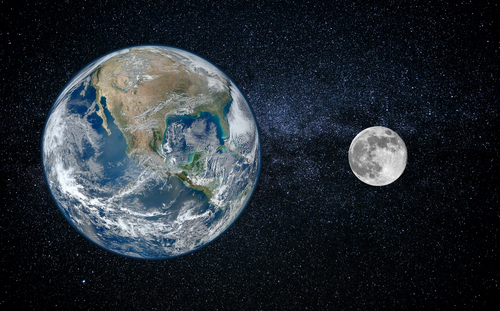
\includegraphics[scale=1.3]{Imagenes/Fuerza_09.jpg}
\end{figure}
\end{frame}

\subsection{Representación de una fuerza}

\begin{frame}
\frametitle{Representación de una fuerza}
Para describir una fuerza vectorial debemos indicar:
\setbeamercolor{item projected}{bg=aquamarine,fg=black}
\setbeamertemplate{enumerate items}{%
\usebeamercolor[bg]{item projected}%
\raisebox{1.5pt}{\colorbox{bg}{\color{fg}\footnotesize\insertenumlabel}}%
}
\begin{enumerate}[<+->]
\item Su dirección de acción.
\item Su magnitud, \pause es decir, la cantidad que describe \enquote{cuánto} o \enquote{qué tan tanto} la fuerza empuja o tira.
\end{enumerate}
\end{frame}
\begin{frame}
\frametitle{Unidad de la fuerza}
La unidad que mide la magnitud de fuerza en el Sistema Internacional, es el \textocolor{alizarin}{newton}, que se abrevia \unit{\newton}.
\end{frame}
\begin{frame}
\frametitle{¿Qué representa un newton?}
El newton representa la unidad de fuerza necesaria para que un objeto de \textocolor{blue}{un kilogramo}, obtenga una aceleración de \textocolor{blue-violet}{un metro por segundo al cuadrado}:
\pause
\begin{align*}
\unit{\newton} \hspace{0.5cm} \Rightarrow \hspace{0.5cm} \left[ \unit[per-mode=fraction]{\kilo\gram\meter\per\square\second} \right]
\end{align*}
\end{frame}

\section{Suma de fuerzas}

\begin{frame}
\frametitle{Más de una fuerza actuando}
Los experimentos muestran que si dos fuerzas y actúan al mismo tiempo en un punto A de un cuerpo, \pause el efecto sobre el movimiento del cuerpo \textocolor{burgundy}{es igual al de una sola fuerza} igual a la suma vectorial de las fuerzas originales.
\end{frame}
\begin{frame}
\frametitle{Suma vectorial}
El resultado de la suma vectorial, es $\va{R}$, \pause es el \textocolor{cinnabar}{vector resultante}.
\pause
\begin{figure}
    \centering
    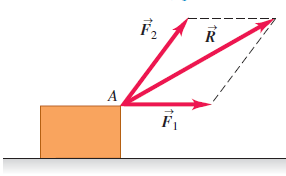
\includegraphics[scale=0.8]{Imagenes/Fuerza_06.png}
\end{figure}
\end{frame}
\begin{frame}
\frametitle{Para el caso con más fuerzas}
En general, el efecto de cualquier cantidad de fuerzas aplicadas a un punto de un cuerpo es el mismo de una sola fuerza igual a la suma vectorial de las fuerzas.
\end{frame}
\begin{frame}
\frametitle{Principio importante en física}
Éste es el importante \textocolor{coolblack}{principio de superposición de fuerzas}.
\end{frame}
\begin{frame}
\frametitle{Uso de un tema revisado}
Como la fuerza es un vector, podemos estudiarla a partir de las componentes vectoriales, \pause tal y como lo vimos en el tema de vectores.
\end{frame}
\begin{frame}
\frametitle{Componentes de una fuerza}
Para un vector que forma un ángulo con respecto a la horizontal, se tiene que:
\pause
\begin{figure}
    \centering
    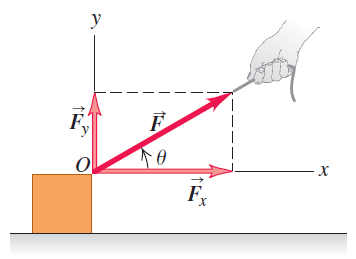
\includegraphics[scale=0.7]{Imagenes/Fuerza_07.png}
\end{figure}
\end{frame}
\begin{frame}
\frametitle{Componentes de una fuerza}
Las componentes $F_{x}$ y $F_{y}$ tienen juntas el mismo efecto que la fuerza original $\va{F}$.
\pause
\begin{figure}
    \centering
    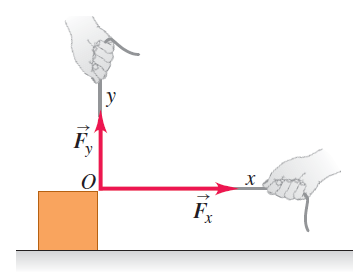
\includegraphics[scale=0.65]{Imagenes/Fuerza_08.png}
\end{figure}
\end{frame}
\begin{frame}
\frametitle{Un sistema de fuerzas}
Para resolver en una fuerza resultante, trabajamos con los vectores como lo hicimos en el tema anterior:
\pause
\setbeamercolor{item projected}{bg=red,fg=white}
\setbeamertemplate{enumerate items}{%
\usebeamercolor[bg]{item projected}%
\raisebox{1.5pt}{\colorbox{bg}{\color{fg}\footnotesize\insertenumlabel}}%
}
\begin{enumerate}[<+->]
\item Tabla de vectores por cuadrante, magnitud y ángulo.
\item Tabla de componentes por vector en el eje $x$ y en el eje $y$.
\seti
\end{enumerate}
\end{frame}
\begin{frame}
\frametitle{Un sistema de fuerzas}
\setbeamercolor{item projected}{bg=red,fg=white}
\setbeamertemplate{enumerate items}{%
\usebeamercolor[bg]{item projected}%
\raisebox{1.5pt}{\colorbox{bg}{\color{fg}\footnotesize\insertenumlabel}}%
}
\begin{enumerate}[<+->]    
\conti
\item Obtener la magnitud del vector resultante.
\item Obtener el ángulo del vector resultante.
\end{enumerate}
\end{frame}
\begin{frame}
\frametitle{Tabla de vectores}
\begin{table}
\centering
\begin{tabular}{c | c | c | c}
Vector & Cuadrante & Magnitud & Ángulo \\ \hline
$F_{1}$ & & & \\ \hline
$F_{2}$ & & & \\ \hline
$\ldots$ & & & \\ \hline 
\end{tabular}
\end{table}
\end{frame}
\begin{frame}
\frametitle{Tabla de componentes}
\begin{table}
\centering
\begin{tabular}{c | c | c | c}
Componente & Expresión & Sustitución & Valor \\ \hline
$F_{1x}$ & & & \\ \hline
$F_{1y}$ & & & \\ \hline    
$F_{2x}$ & & & \\ \hline
$F_{2y}$ & & & \\ \hline    
\end{tabular}
\end{table}
\end{frame}
\begin{frame}
\frametitle{Componentes de la resultante}
Las componentes $R_{x}$ y $R_{y}$ del vector resultante son:
\pause
\begin{eqnarray*}
\begin{aligned}
R_{x} = \nsum_{i=1}^{n} F_{ix} \\[0.5em] \pause
R_{y} = \nsum_{i=1}^{n} F_{iy}
\end{aligned}
\end{eqnarray*}
\end{frame}
\begin{frame}
\frametitle{Magnitud dl vector fuerza resultante}
La magnitud del vector fuerza resultantes es:
\pause
\begin{eqnarray*}
\begin{aligned}
\abs{\va{R}} = \pause \sqrt{(R_{x})^{2} + (R_{y})^{2}}
\end{aligned}
\end{eqnarray*}
\end{frame}
\begin{frame}
\frametitle{Ángulo del vector fuerza resultante}
El ángulo que determina la dirección del vector fuerza resultante es:
\pause
\begin{align*}
\theta_{R} = \tan^{-1} \left( \dfrac{R_{y}}{R_{x}} \right)
\end{align*}
\end{frame}

\section{Dinámica}
\frame{\tableofcontents[currentsection, hideothersubsections]}
\subsection{Introducción}

\begin{frame}
\frametitle{Preguntas disparadoras}
¿Cuáles son las causas del movimiento? 
\end{frame}
\begin{frame}
\frametitle{Preguntas disparadoras}
¿Cómo puede un remolcador empujar un trasatlántico que es mucho más pesado que él?
\pause
\begin{figure}
    \centering
    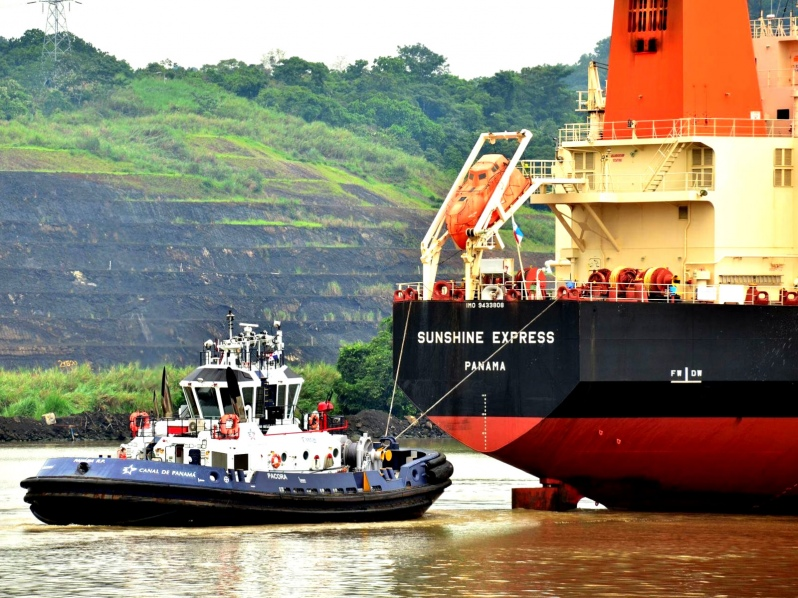
\includegraphics[scale=0.2]{Imagenes/Fuerza_10.jpg}
\end{figure}
\end{frame}
\begin{frame}
\frametitle{Preguntas disparadoras}
¿Por qué es más difícil controlar un automóvil en hielo mojado que en concreto seco?
\begin{figure}
    \centering
    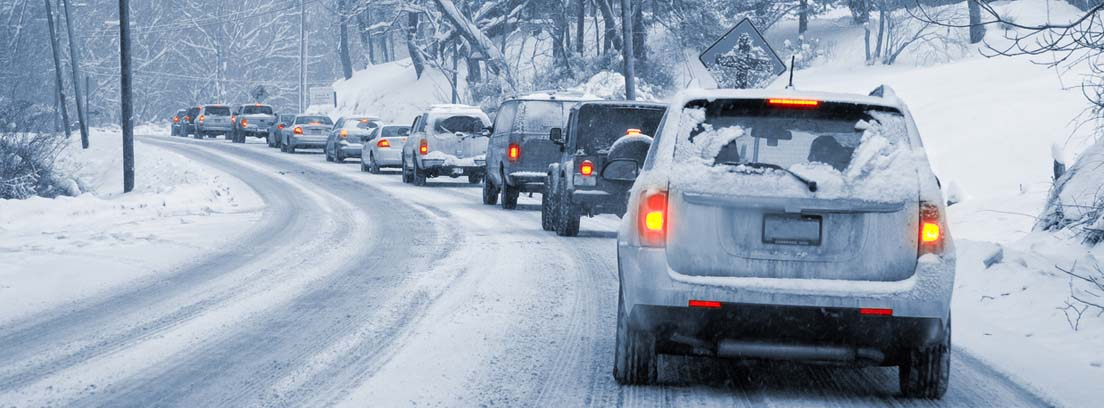
\includegraphics[scale=0.2]{Imagenes/Fuerza_11.jpg}
\end{figure}
\end{frame}
\begin{frame}
\frametitle{Respuestas a las Preguntas}
Las respuestas a estas preguntas y a otras similares nos llevan al tema de la \textocolor{coquelicot}{dinámica}, \pause es decir, la relación entre el movimiento y las fuerzas que lo causan.
\end{frame}
\begin{frame}
\frametitle{Conceptos necesarios}
Para apoyar nuestra revisión, utilizaremos los conceptos de \textocolor{cordovan}{fuerza} y la \textocolor{darkcyan}{masa}, para analizar los principios de la dinámica.
\end{frame}
\begin{frame}
\frametitle{Masa y peso}
Recordemos que:
\setbeamercolor{item projected}{bg=deepchampagne,fg=black}
\setbeamertemplate{enumerate items}{%
\usebeamercolor[bg]{item projected}%
\raisebox{1.5pt}{\colorbox{bg}{\color{fg}\footnotesize\insertenumlabel}}%
}
\begin{enumerate}[<+->]
\item Masa es la cantidad de sustancia que contiene un cuerpo, \pause en el sistema MKS su unidad es el \unit{\kilo\gram}, \pause en el sistema cgs, la unidad es el \unit{\gram}.
\seti
\end{enumerate}
\end{frame}
\begin{frame}
\frametitle{Masa y peso}
\setbeamercolor{item projected}{bg=deepchampagne,fg=black}
\setbeamertemplate{enumerate items}{%
\usebeamercolor[bg]{item projected}%
\raisebox{1.5pt}{\colorbox{bg}{\color{fg}\footnotesize\insertenumlabel}}%
}
\begin{enumerate}[<+->]
\conti
\item Peso es la masa multiplicada por el valor de \textbf{g}, \pause la aceleración debida a la gravedad: \SI{9.81}{\meter\per\square\second}, \pause las unidades del peso son los Newtons (\unit{\newton})
\pause
\begin{align*}
W = m \, g \hspace{0.5cm} \Rightarrow \hspace{0.5cm} \left[ \unit{\newton} \right]
\end{align*}
\end{enumerate}
\end{frame}    
\begin{frame}
\frametitle{Los primeros principios}
Estos principios se establecieron en sólo tres leyes que fueron claramente enunciadas por Sir Isaac Newton.
\begin{figure}
    \centering
    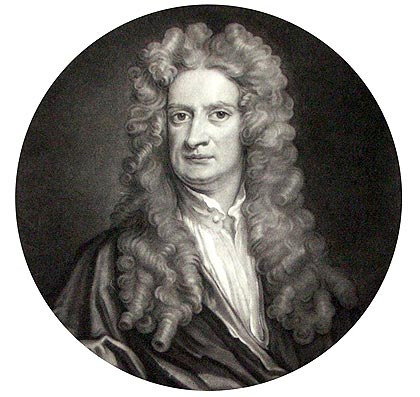
\includegraphics[scale=0.35]{Imagenes/Newton.jpg}
\end{figure}
\end{frame}

\section{Las leyes de Newton}
\frame{\tableofcontents[currentsection, hideothersubsections]}
\subsection{Primera ley}

\begin{frame}
\frametitle{Ley de la inercia}
Un cuerpo sobre el que no actúa una fuerza neta se mueve con velocidad constante (que puede ser cero) y aceleración cero.
\end{frame}
\begin{frame}
\frametitle{La ley de la inercia}
Un objeto en reposo permanece en reposo \pause y un objeto en movimiento, continuará en movimiento con una velocidad constante \pause a menos que se aplique una fuerza externa neta para modificar dicho estado.
\end{frame}
\begin{frame}
\frametitle{Ejemplo de la primera ley}
\begin{figure}
    \centering
    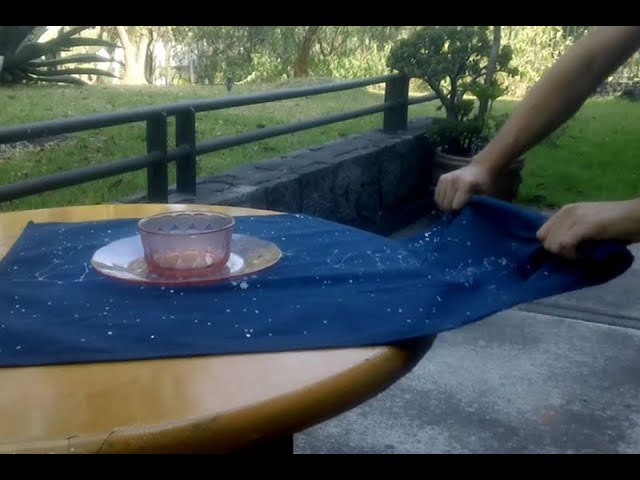
\includegraphics[scale=0.35]{Imagenes/Newton_01.jpg}
\end{figure}
\end{frame}
\begin{frame}
\frametitle{Concepto de inercia}
La tendencia de un cuerpo a seguir moviéndose una vez iniciado su movimiento es resultado de una propiedad llamada \textocolor{darkmagenta}{inercia}.
\end{frame}

\subsection{Segunda ley}

\begin{frame}
\frametitle{Fuerza sobre un cuerpo}
Si una \textocolor{darkscarlet}{fuerza externa neta} actúa sobre un cuerpo, éste se acelera.
\\
\bigskip
\pause
La dirección de aceleración es la misma que la dirección de la fuerza neta. 
\end{frame}
\begin{frame}
\frametitle{Expresión para la segunda ley}
El vector de fuerza neta es igual a la masa del cuerpo multiplicada por su aceleración.
\pause
\begin{align*}
\va{F} = m \, \va{a}
\end{align*}
\end{frame}
\begin{frame}
\frametitle{La segunda ley de Newton}
La segunda ley de Newton es una ley fundamental de la naturaleza, \pause \textocolor{darkslateblue}{la relación básica entre fuerza y movimiento}.
\end{frame}
\begin{frame}
\frametitle{El triángulo de la fuerza}
Ocupamos una referencia gráfica para el uso de la segunda ley de Newton: \pause \textocolor{debianred}{el triángulo de la fuerza}:
\pause
\begin{figure}
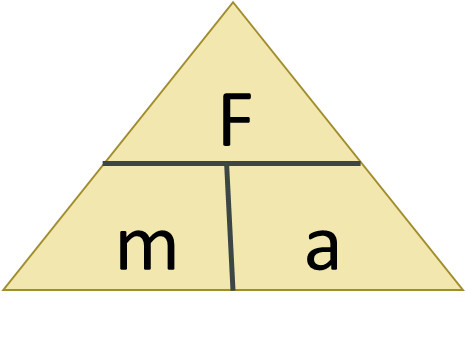
\includegraphics[scale=1]{Imagenes/Newton_11.jpg}
\end{figure}
\end{frame}
\begin{frame}
\frametitle{Ejercicio con la segunda ley}
Un trabajador aplica una fuerza horizontal constante con magnitud de \SI{20}{\newton} a una caja con masa de \SI{40}{\kilo\gram} que descansa en un piso plano con fricción despreciable.
\\
\bigskip
\pause
¿Qué aceleración experimenta la caja?.
\end{frame}
\begin{frame}
\frametitle{Entendiendo el ejercicio}
\begin{figure}
    \centering
    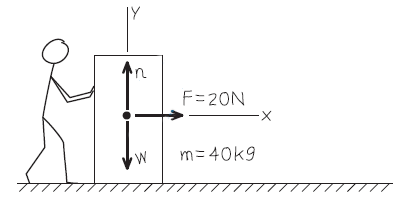
\includegraphics[scale=1]{Imagenes/Newton_02.png}
\end{figure}
\end{frame}
\begin{frame}
\frametitle{Resolviendo el ejercicio}
\textocolor{red}{Datos:}
\pause
\begin{align*}
F &= \SI{20}{\newton} \\[0.5em]
m &= \SI{40}{\kilo\gram}
\end{align*}
\end{frame}
\begin{frame}
\frametitle{Resolviendo el ejercicio}
\textocolor{red}{Expresión:}
\pause
\begin{figure}
    \centering
    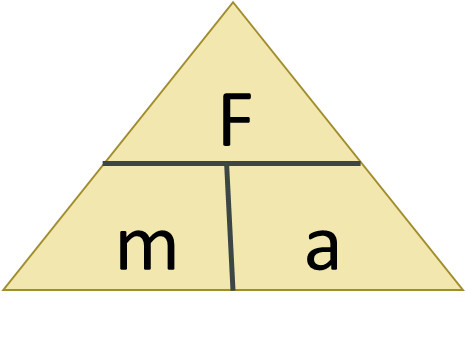
\includegraphics[scale=1]{Imagenes/Newton_11.jpg}
\end{figure}
\pause
\begin{align*}
a = \dfrac{F}{m}
\end{align*}
\end{frame}
\begin{frame}
\frametitle{Resolviendo el ejercicio}
\textocolor{red}{Sustitución:}
\pause
\begin{eqnarray*}
\begin{aligned}
a &= \dfrac{F}{m} = \pause \dfrac{\SI{20}{\newton}}{\SI{40}{\kilo\gram}} = \\[0.5em] \pause
a &= 0.5 \, \dfrac{\dfrac{\unit{\kilo\gram\meter}}{\unit{\square\second}}}{\unit{\kilo\gram}} = \\[0.5em] \pause 
a &= 0.5 \, \dfrac{\unit{\kilo\gram\meter}}{\unit{\kilo\gram\square\second}} = \pause \SI[per-mode=fraction]{0.5}{\meter\per\square\second}
\end{aligned}
\end{eqnarray*}
\end{frame}
\begin{frame}
\frametitle{Sobre las unidades}
Conviene aclarar que en el sistema \textbf{MKS}, \pause se utilizan las unidades de metro, kilogramo y segundo, como unidades de longitud, masa y tiempo, respectivamente.
\end{frame}
\begin{frame}
\frametitle{Sobre las unidades}
En ciencia e ingeniería se utiliza también un sistema llamado \textbf{cgs}, \pause donde las unidades de longitud, masa y tiempo son: el centímetro, gramo y segundo.
\end{frame}
\begin{frame}
\frametitle{Unidad de fuerza en cgs}
La unidad de medida de la fuerza en el sistema \textbf{cgs}, es la llamada \textocolor{denim}{dina}:
\pause
\begin{align*}
1 \, \text{dina} = \SI[per-mode=fraction]{1}{\gram\centi\meter\per\square\second}
\end{align*}
Sería conveniente que construyas el factor de conversión de dinas a Newtons.
\end{frame}
\begin{frame}
\frametitle{Unidad de fuerza sistema inglés}
En el sistema británico, las unidades de:
\pause
\setbeamercolor{item projected}{bg=ferrarired,fg=white}
\setbeamertemplate{enumerate items}{%
\usebeamercolor[bg]{item projected}%
\raisebox{1.5pt}{\colorbox{bg}{\color{fg}\footnotesize\insertenumlabel}}%
}
\begin{enumerate}[<+->]
\item Fuerza es la \textocolor{ao}{libra} (o libra-fuerza).
\item Masa es el \textocolor{electricindigo}{slug}.
\item Aceleración es el pie por segundo al cuadrado.
\end{enumerate}
\end{frame}
\begin{frame}
\frametitle{Unidad de fuerza sistema inglés}
Así que la unidad de fuerza en el sistema inglés es:
\pause
\begin{align*}
1 \, \text{libra-fuerza} = \text{slug} \, \dfrac{\text{pie}}{\unit{\square\second}}
\end{align*}

\end{frame}
\end{document}